\begin{frame}[allowframebreaks]{PixelCNN}
\textbf{Masked Spatial (2D) Convolution - PixelCNN}
\begin{itemize}
    \item Images can be flattened into 1D vectors, but they are fundamentally 2D.
    \item We can use a masked variant of ConvNet to exploit this knowledge.
    \item First, we impose an autoregressive ordering on 2D images:
\end{itemize}

\begin{figure}
    \centering
    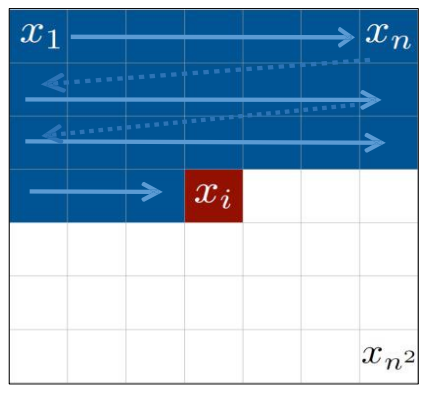
\includegraphics[height=0.4\textheight, width=\textwidth,keepaspectratio]{images/arm/raster-scan.png}
    \caption{Raster scan ordering of a 2D image. The pixels are processed in a left-to-right, top-to-bottom manner, similar to reading text.}
\end{figure}

\framebreak
\begin{itemize}
    \item The autoregressive ordering allows us to use a convolutional neural network (CNN) to predict the next pixel based on the previously generated pixels.
    \item We use masked convolutions to ensure that the model only has access to the pixels that have already been generated.
    \item The convolutional layers are designed to respect the autoregressive ordering, meaning that each pixel is predicted based on its left and top neighbours, but not the right or bottom neighbours.
\end{itemize}
\framebreak
\textbf{PixelCNNs}: Use the neighbour pixels to predict the new pixel.
\begin{columns}
        \begin{column}{0.5\textwidth}
            \begin{figure}
                \centering
                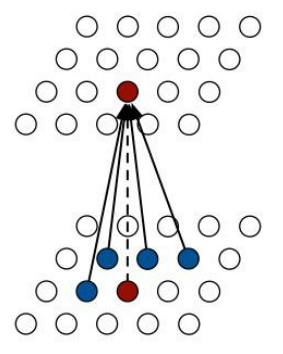
\includegraphics[width=0.9\textwidth, keepaspectratio]{images/arm/pixelcnn.png}
                \caption{Image generation with pixelCNN}
            \end{figure}
        \end{column}
        \begin{column}{0.5\textwidth}
            \begin{figure}
                \centering
                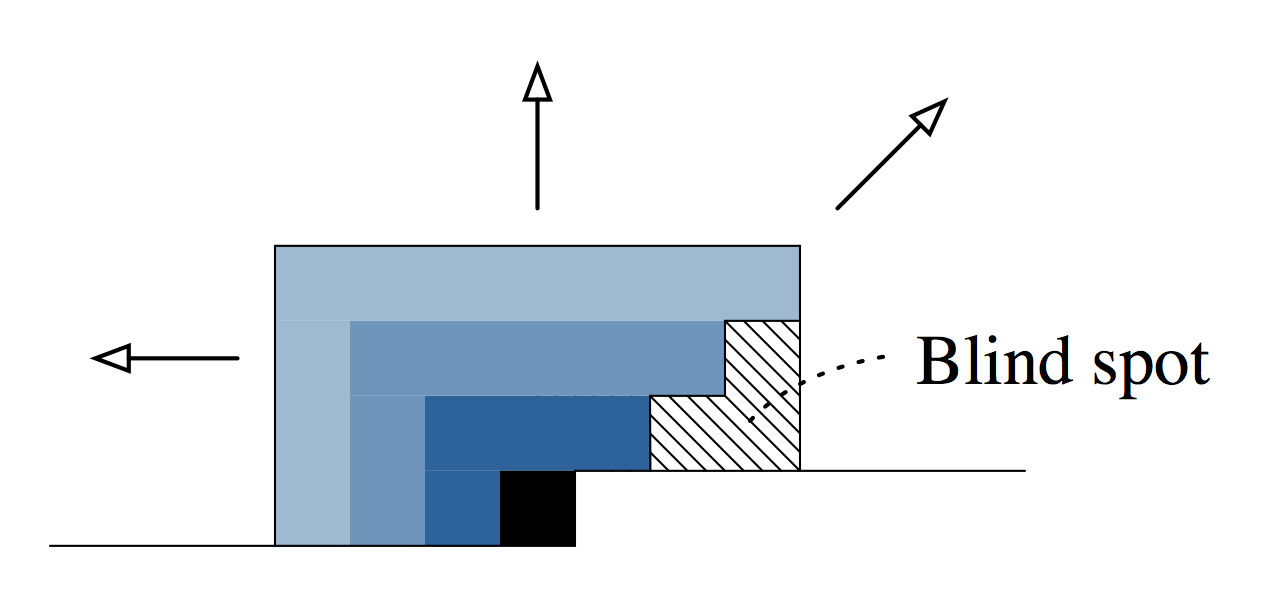
\includegraphics[width=1.1\textwidth,keepaspectratio]{images/arm/pixelcnn-blindspot.png}
                \caption{PixelCNN-style masking has one problem: blind spot in receptive field. The model cannot see the pixels to the right and below the current pixel, which can lead to artifacts in generated images.}
            \end{figure}
        \end{column}
    \end{columns}

\framebreak

\begin{itemize}
    \item PixelCNN results
        \begin{figure}
        \centering
        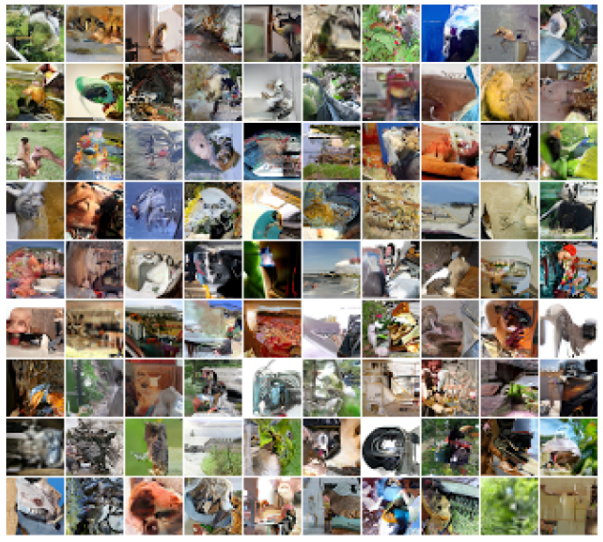
\includegraphics[height=0.65\textheight, width=\textwidth, keepaspectratio]{images/arm/pixelcnn_results.png}
        \caption{Image generation with pixelCNN. Model trained on Imagenet (32 x 32 pixels)}
    \end{figure}
\end{itemize}
\end{frame}